\section{Конструкторский раздел}

\subsection{Описание сущностей проектируемой базы данных}

В базе данных будет существовать 5 сущностей и 6 таблиц, одна из которых является развязочной. 
\begin{figure}[hbtp]
	\centering
	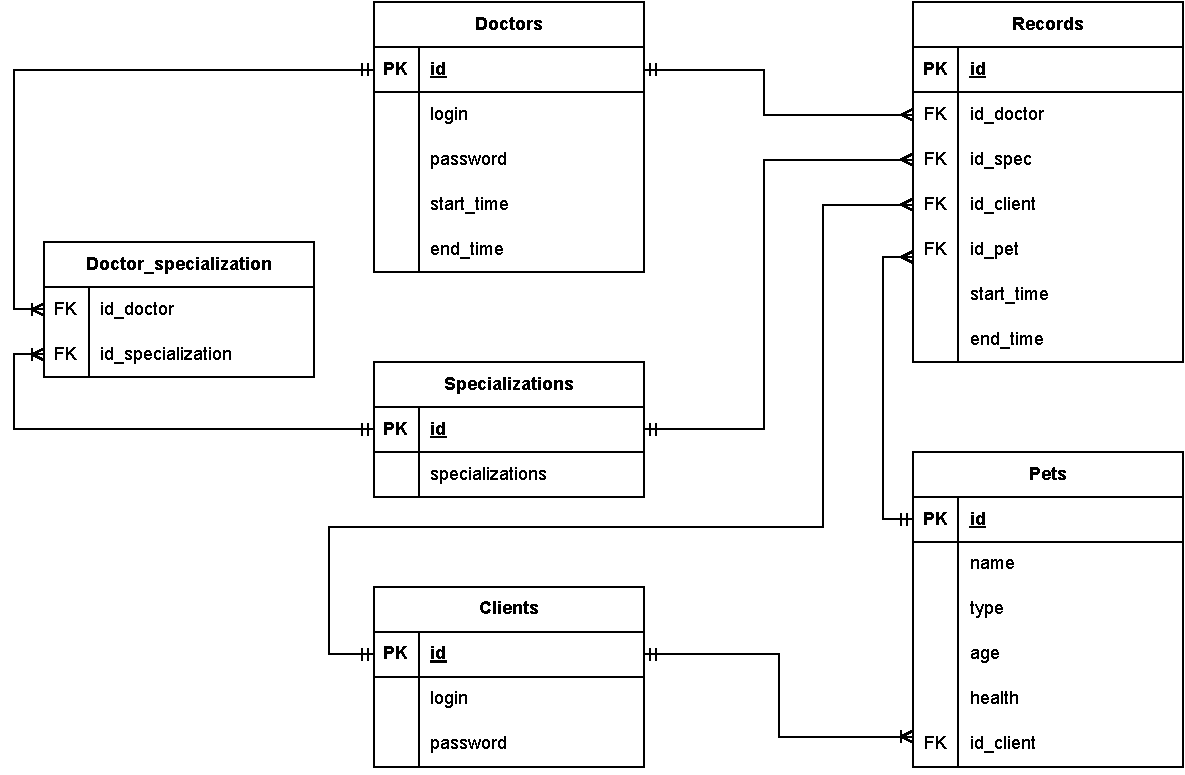
\includegraphics[width=170mm]{image/bd.pdf}
	\caption{Диаграмма проектируемой базы данных}
	\label{img:idef}
\end{figure}

Необходимы следующие таблицы.
\begin{enumerate}[label=\arabic*)]
	\item Таблица c работниками клиники, то есть докторами (Doctors).
	\item Таблица для специализаций работников клиники (Specializations).
	\item Развязочная таблица для работников и их специализаций.
	\item Таблица c клиентами клиники (Clients).
	\item Таблица c питомцами клиники (Pets).
	\item Таблица c записями на прием (Records).
\end{enumerate}

В таблице \ref{tab:doctors}  описаны поля таблицы Doctors. В таблице \ref{tab:specializations} описаны поля таблицы Specializations. В таблице \ref{tab:DC} описаны поля таблицы связки для Doctors и Specializations. 
\begin{table}[hbtp]
	\begin{center}
			\caption{\label{tab:doctors}Поля таблицы Doctors}
		\begin{tabular}{|l|l|l|l|l|l|}
			\hline {Поле} & {Тип данных} & {Описание}  \\ \hline
			id\_doctor  & serial & Идентификатор работника   \\ \hline
			login & text & Идентификатор работника для входа в систему \\ \hline
			password & text & Пароль работника для входа в систему  \\ \hline
			start\_time & int & Начало рабочих часов\\ \hline
			end\_time & int & Конец рабочих часов\\ \hline
		\end{tabular}
	\end{center}
\end{table}

\begin{table}[hbtp]
	\begin{center}
		\caption{\label{tab:specializations}Поля таблицы Specializations}
		\begin{tabular}{|l|l|l|l|l|l|}
			\hline {Поле} & {Тип данных} & {Описание}  \\ \hline
			id\_spec  & serial & Идентификатор специализации \\ \hline
			spec\_name & text & Название специализации\\ \hline
		\end{tabular}
	\end{center}
\end{table}

\begin{table}[hbtp]
	\begin{center}
		\caption{\label{tab:DC}Поля развязочной таблицы Doctors-Specializations}
		\begin{tabular}{|l|l|l|l|l|l|}
			\hline {Поле} & {Тип данных} & {Описание}  \\ \hline
			id\_doctor  & int & Идентификатор доктора \\ \hline
			id\_specialization & int & Идентификатор специализации \\ \hline
		\end{tabular}
	\end{center}
\end{table}

В таблице~\ref{tab:clients} описаны поля таблицы Clients. Клиенты и работники имеют 3 одинаковых поля, но они разнесены по разным таблицам, ибо у них разные роли в бизнес-процессах. Разделение позволяет лучше структурировать информацию и дополнительные связи с другими сущностями.
\begin{table}[hbtp]
	\begin{center}
		\caption{\label{tab:clients}Поля таблицы Clients}
		\begin{tabular}{|l|l|l|l|l|l|}
			\hline {Поле} & {Тип данных} & {Описание}  \\ \hline
		id\_client  & serial & Идентификатор клиента   \\ \hline
		login & text & Идентификатор клиента для входа в систему \\ \hline
		password & text & Пароль клиента для входа в систему  \\ \hline
		\end{tabular}
	\end{center}
\end{table}

 В таблице \ref{tab:pets}  описаны поля таблицы Pets. В данном проекте у питомца может быть только один владелец, но у владельца может быть много питомцев. Поэтому информация о связи питомец-владелец реализуется с помощью таблицы Pets, где содержится идентификатор хозяина. В таблице \ref{tab:records}  описаны поля таблицы Records, которая хранит записи на приемы. 
 
\begin{table}[hbtp]
	\begin{center}
			\captionsetup{justification=raggedright, singlelinecheck=false}
			\caption{\label{tab:pets}Поля таблицы Pets}
		\begin{tabular}{|l|l|l|l|l|l|}
			\hline {Поле} & {Тип данных} & {Описание}  \\ \hline
			id\_pet  & serial & Идентификатор питомца   \\ \hline
			name & text & Кличка питомца \\ \hline
			type & text & Вид, порода питомца  \\ \hline
			age & int & Возраст питомца \\ \hline
			health & int & Уровень здоровья питомца  \\ \hline
			id\_client & int & Идентификатор хозяина  \\ \hline
		\end{tabular}
	\end{center}
\end{table}

\begin{table}[hbtp]
		\caption{\label{tab:records}Поля таблицы Records}
	\begin{center}
		\begin{tabular}{|l|l|l|l|l|l|}
			\hline {Поле} & {Тип} & {Описание}  \\ \hline
			id\_record  & serial & Идентификатор приема   \\ \hline
			id\_doctor & int & Идентификатор доктора  \\ \hline
			id\_spec & int & Идентификатор специализации доктора  \\ \hline
			id\_pet & int & Идентификатор питомца   \\ \hline
			start\_time & int & Время начала приема\\ \hline
			end\_time & int & Время конца приема\\ \hline
		\end{tabular}
	\end{center}
\end{table}

\pagebreak

\subsection{Ролевая модель}
Исходя из сценариев приложения, представленных на рисунке \ref{img:use-case} можно выделить следующие роли.
\begin{enumerate}[label=\arabic*)]
	\item Гость. Имеет права только на просмотр таблиц сотрудников и их специализаций.
	\item Клиент. Имеет права на просмотр и изменение записей, связанных с ним и его питомцами в соответствующих таблицах. Как и гость может смотреть список сотрудников и их специализаций.
	\item Работник. Имеет права на просмотр всех таблиц, кроме таблицы с клинтами. В таблице с клиентам не может получать доступ к паролю клиента, то есть поле password. Может изменять данные о себе, о записях на приемы и о питомцах, связанных с ним.
	\item Администратор. Имеет права на создание и обновление всех таблиц.
\end{enumerate}

\subsection{Триггер базы данных}

Для добавления новой записи на прием нужно убедиться, что она корректна. Для этого необходим триггер, реализующий анализ уже существующих записей в таблице для проверки соответствия желаемого времени графику работы доктора и его доступности. При попытке добавления новой записи в таблицу Records вызывается функция, схема алгоритма работы которой представлена на рисунке~\ref{img:tr}.

\begin{figure}[hbtp]
	\centering
	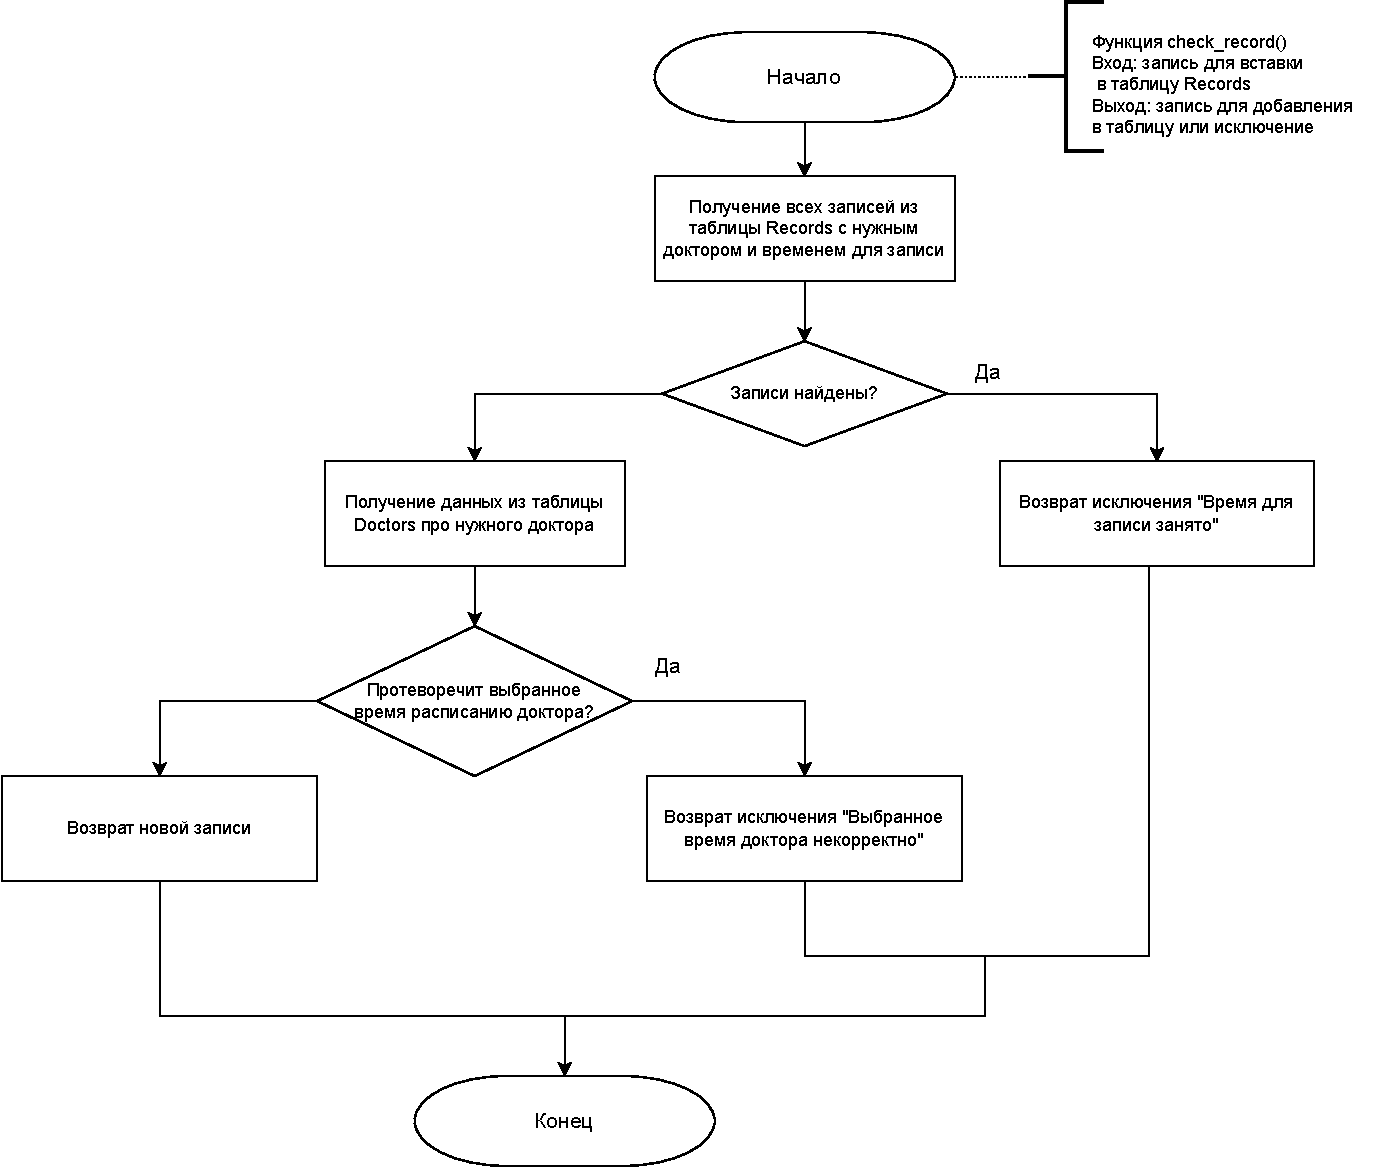
\includegraphics[width=\textwidth]{image/tr.pdf}
	\caption{Схема алгоритма функции проверки новой записи check\_record()}
	\label{img:tr}
\end{figure}


\subsection*{Вывод}
В данном разделе были описаны сущности, ролевая модель и функции проектируемой базы данных.